\chapter{Hardware Description}
\label{ch:Hardware}
Along this chapter we will introduce a general description of all devices used to gather data for the development of this project.


It should be noted at this point that there are two clearly differentiated parts. In the first one, we work with Force Plate and GaitWatch data, taking out their characteristic signals and synchronising them. In the second one, we work jointly with Gait Watch and Qualisys System data for the purpose of comparing the accuracy in the calculated orientation angles.


\section{GaitWatch}

GaitWatch is an Inertial Measurement Unit (IMU) designed for gait monitoring of patients. It was developed by Prof. Dr. Med. Kai Bötzel at the Department of Neurology of Ludwig-Maximilians University in Munich in conjunction with Dr. Alberto Olivares Vicente from the Department of Signal Theory, Telematics and Communications of the University of Granada. \cite{OlivaresBotzel2013}.

The system is composed of the central processing unit and a set of measuring units which are wired to it. The measuring units are placed in the patients’ thighs, shanks, arms and trunk.

The central processing unit has a microcontroller which is in charge of gathering the data from the external measurement units and writing them to the memory card. So, this central unit is placed on the trunk inside a box and it contains an AL-XAVRB board with an AVRATxmega processor which contains the necessary embedded firmware to gather the data from all the measurement units and store them in a microSD card. Also, the trunk box contains some embedded magnetic and inertial sensors.

\begin{figure}[H]
	\centering
	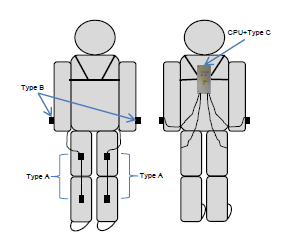
\epsfig{file=imagenes/GeneralDiagramGW, width=9cm}
	\caption{General Diagram of the Gait Watch.}
	\label{fig:diagram}
\end{figure}

\begin{figure}[H]
	\centering
	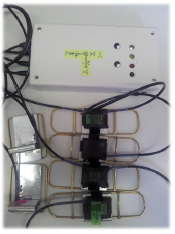
\epsfig{file=imagenes/devicesGW, width=7cm, angle = 90}
	\caption{Devices used in Gait Watch System.}
	\label{fig:devicesGW}
\end{figure}

There are three different kinds of external units with the following components:
\begin{itemize}
	\item Type A (thighs and shanks): 
	\begin{itemize}
		\item IMU 5 from Sparkfun. IMU 5 contains an IDG500  biaxial gyroscope (from which only Y axis is actually used) with a measurement range of $\pm500deg/s$ and a $\pm3g$ triaxial accelerometer, ADXL335 .
	\end{itemize}
	\item Type B (arms):
	\begin{itemize}
		\item IDG500  biaxial $\pm500deg/s$ gyroscope.
	\end{itemize}
	\item Type C (trunk box):
	\begin{itemize}
		\item ADXL345  triaxial accelerometer with programmable range ($\pm16g/\pm8g/\pm4g/\pm2g$).
		\item IMU3000 triaxial gyroscope with programmable range ($\pm250/\pm500/\pm1000/\pm3000 (deg/s)$).
		\item Micromag3  triaxial magnetometer ($\pm11Gauss$).
	\end{itemize}
\end{itemize}


\section{Force Platform}
Force Plate (FDM-S Multifunction Force-measuring Plate, Zebris) is a System for force measurement and it can be used as a complete measuring unit for stance and roll-off analysis \cite{forceplate}.

This platform consist of a large number of force sensors and enables the distribution of static and dynamic forces under the feet to be analyzed during stance and gait (65x40 cells of sensors). As a result, foot deformities, foot function and posture can be analysed and are available as an evaluation report \cite{forceplate}.

Therefore, this gathered information can be used afterwards to analyse the postural adjustments with the right software.

\begin{figure}[H]
	\centering
	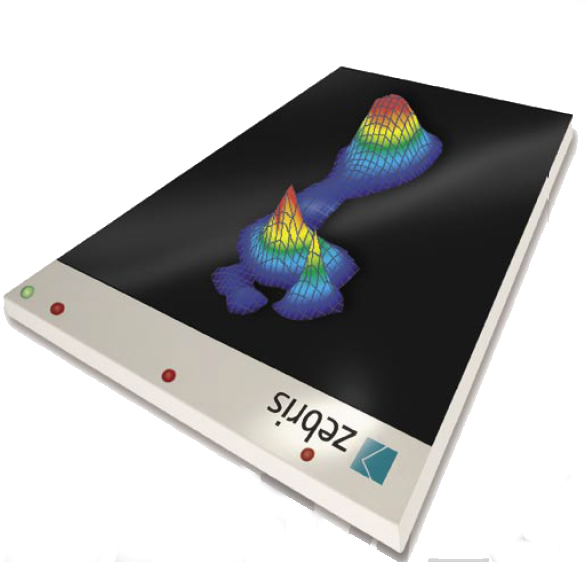
\epsfig{file=imagenes/FDMS_Zebris, width=7cm}
	\caption{Platform used to analyse the force under the feet.}
	\label{fig:FDMS}
\end{figure}


\section{Qualisys System}
The Qualisys optical motion tracker is a system that uses high speed digital cameras to capture the motion of a measurement object with passive or active markers attached \cite{OlivaresBotzel2013}.

This technology is used by researchers and clinicians to understand the basics of human motion or improve treatment during a rehabilitation process. Also, it used in industrial applications, for example, interior design of a car can be improved by using this System to evaluate the comfort and safety factors for the car driver \cite{Qualisys}.

The technology is precise and delivers high quality data to the observer in real-time. The core component of the Qualisys System is one or more infrared optical cameras that emit a beam of infrared light. Also, there are small retro-reflective markers on a object or person. When the cameras emit infrared light onto the markers, these reflect the light back to the camera sensor and this information is used to calculate the position with high spatial resolution  \cite{Qualisys}. The used system has eight cameras which are distributed around a room.

\begin{figure}[H]
	\centering
	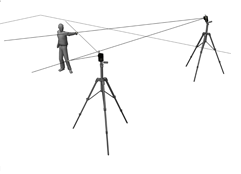
\epsfig{file=imagenes/QualysisSystem, width=7cm}
	\caption{Qualisys optical motion tracker.}
	\label{fig:QS}
\end{figure}

The provided software tools allows to perform basic motion calculations, such as speed, acceleration, rotation and angle, as well as other more complex calculations. The precision of this system allows its use as a reference system to evaluate portable motion tracking systems such as the GaitWatch  \cite{OlivaresBotzel2013}.
